%%% MATH COMMANDS %%%
\newcommand{\R}{\ensuremath{\mathbb{R}}}
\newcommand{\RNum}[1]{\uppercase\expandafter{\romannumeral #1\relax}}
\def\intavg{\,\ThisStyle{\ensurestackMath{%
    \stackinset{c}{0\LMpt}{c}{0\LMpt}{\SavedStyle-}{\SavedStyle\phantom{\int}}}%
    \setbox0=\hbox{$\SavedStyle\int\,$}\kern-\wd0}\int}
%%%%%%%%%%%%%%%%%%%%%

\documentclass[12pt]{artikel1}
\usepackage{scalerel}
\usepackage[usestackEOL]{stackengine}
\usepackage{pgfplots}
\pgfplotsset{compat=1.18}
\usepackage{amsmath}
\usepackage{amsthm}
\usepackage{tikz}
\usetikzlibrary{3d}
\usepackage[utf8]{inputenc}
\usepackage{graphicx}
\usepackage[english]{babel}
\usepackage[a4paper, margin=3cm]{geometry}
\usepackage[T1]{fontenc}
\sffamily
\usepackage{textpos}
\usepackage{amssymb}
\usepackage{listings}
\usepackage{eurosym}
\usepackage{ragged2e}
\usepackage{blindtext}
\usepackage{romannum}
\usepackage[
    backend=biber,
    style=apa,
  ]{biblatex}
\usepackage[most]{tcolorbox}
\addbibresource{PDE.bib}
\usepackage{hyperref}
\hypersetup{
    pdfpagemode=UseNone, 
    colorlinks=true,
    filecolor=blue,
    linkcolor=red,
    citecolor=black,
    urlcolor=blue
}
\DeclareAutoCiteCommand{textcite}{\textcite}{\textcites}
\ExecuteBibliographyOptions{autocite=textcite}
\linespread{1.25}
\DeclareMathOperator*{\argmax}{arg\,max}
\newtheorem{proposition}{Proposition}[section]
\newtheorem{theorem}{Theorem}[section]
\newtheorem{corollary}{Corollary}[theorem]
\newtheorem{lemma}[theorem]{Lemma}
\newtheorem{definition}{Definition}[section]

\begin{document}
\pagenumbering{arabic}
\begin{textblock*}{250mm}(0cm,-2cm)
\noindent Partial Differential Equations \RN{2}
\end{textblock*}
\begin{textblock*}{250mm}(.80\textwidth,-2cm)
\noindent Santeri Väätäjä
\end{textblock*}
\vspace*{-2cm}
\section*{Regularity of Elliptic Second Order Partial Differential Equations: Calder\'{o}n-Zygmund estimates}
\vspace*{-.5cm}
\line(1,0){10cm}
\vspace*{.5cm}

\noindent The regularity of solutions to second-order elliptic differential equations refers to the smoothness or differentiability of these solutions. This concept is crucial in the theory of partial differential equations (PDEs) as it determines how well-behaved the solutions are and whether they satisfy the equation in a classical or weak sense.

In order to try to improve the regularity properties, one line of attack that can be taken in the case of second-order elliptic PDEs, and especially in this case with the Laplacian equation, is to examine if the principle that \cite{Fern_ndez_Real_2022} calls ``$u$ is two derivatives more regular than $f$'' holds. The results regarding this phenomenon can be divided into two main results.

\begin{enumerate}
    \item \textit{Schauder estimates:} If $f\in C^{0,\alpha}$ then $u\in C^{2,\alpha}$, for $\alpha\in(0,1)$, or more generally if $f\in C^{k,\alpha}$ then $u\in C^{k+2,\alpha}$.
    \item \textit{Calder\'{o}n-Zygmund estimates:} If $f\in L^p$ then $u\in W^{2,p}$ for $p\in(1,\infty)$.
\end{enumerate}

\noindent From these two, the first one is shown in the lecture notes \cite{covi}, so with interest in expanding the regularity theory of upgrading the weak solutions of the Laplace equation, I will be concentrating on the second item in the list; Calder\'{o}n-Zygmund estimates.

These, unlike Schauder estimates, consider functions in $L^p$-space, so unlike in the first case, we lose the pointwise control of the functions.  Schauder estimates are concerned with the regularity of solutions at each individual point in the domain, requiring that the given data be Hölder continuous. This means that the data must exhibit a certain level of smoothness and continuity pointwise, allowing for precise control over the behavior of the solution at every location. In contrast, Calderón-Zygmund estimates deal with functions that are integrable but may lack pointwise smoothness. These estimates operate within $L^p$-spaces, where the focus is on the overall integrability of the functions rather than their pointwise behavior. As a result, Calderón-Zygmund estimates provide regularity results based on the average properties of the functions, making them applicable even when the data is less regular but still integrable.

I will be restricting the forthcoming analysis to consider only the case where the domain of the Laplacian is assumed to be $\Omega=B_1$, following the analysis done in \cite{covi,Fern_ndez_Real_2022} and \cite{sanpera} which I will be be primarily following on the proofs for Calder\'{o}n-Zygmund estimates. It would be possible to extend the analysis to cover a broader family of domains than the unit ball, but the restriction is made in order to restrict the complexity of the analysis.

\subsection*{Formalization of the Problem}

The problem of establishing some regularity starts by having the Laplacian

\begin{gather}\label{eq:laplacian}
    \begin{cases}
        \Delta u=f,\,x\in B_1 \\
        u=g,\,x\in\partial B_1
    \end{cases}
\end{gather}

\noindent and in the case of Calder\'{o}n-Zygmund estimates we further assume that $f\in L^{p}(B_1)$. Then the estimates give that if $u$ is a weak solution to the problem \ref{eq:laplacian}, then $D^2u\in L^p$ for $p\in (1,\infty)$. The definition of a weak solution is given as follows:

\begin{definition}\label{def:weak}
    A function $u$ is a weak solution of \ref{eq:laplacian} if $u\in H^1(\Omega)$, $u|_{\partial\Omega}=g$ and 
    \begin{gather*}
        \int_\Omega\nabla u\nabla v=\int_\Omega fv
    \end{gather*}
    for all $v\in H^1(\Omega)$ such that $v=0$ in $\partial\Omega$.
\end{definition}

\noindent The proof for this can be treated differently for some specific values of $p$, most notably for $p=2$, which allows a more straightforward proof. It is also noteworthy that the values $1$ and $\infty$ are excluded from the formulation. In these cases, the inclusion of the solution to the $L^p$-space cannot be guaranteed. However, there exist some versions of these estimates that can be given in the case of $L^\infty$. These results are introduced in \cite{sanpera}. This requires introducing new concepts for the function space in which the result applies, namely something called a BMO space. The BMO space is a concept that shares similarities with both Hölder and Sobolev spaces. I will not be concentrating on these estimates, but rather stick with the original bounds for $p$.

To get a better idea of why the estimates hold only for such values of $p$ \cite{Fern_ndez_Real_2022} presents some examples of harmonic functions that exhibit the behavior. In the case for $p=1$, taking the mollified Dirac delta to be the example $f_\epsilon(x)=\epsilon^{-n}\eta(\frac{x}{\epsilon})$ so $f_\epsilon\in C^{\infty}$ and it converges towards the fundamental solution as $\epsilon\rightarrow0$, but that does not belong in the $W^{2,1}$. I have tried to visualize this in figure \ref{fig:failure}.

\begin{figure}[h]
    \centering
    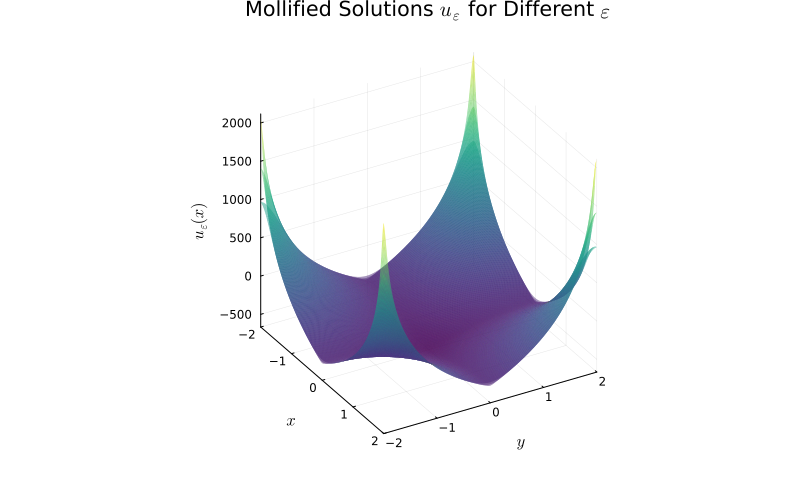
\includegraphics[width=\textwidth]{Laplacian.png}
    \caption{This plot shows the solution $u_\epsilon(x)$ for the Laplacian where the forcing term is a smooth approximation of the Dirac delta function. I used a standard mollifier for this. As the figure shows, the solutions start to diverge as the $\epsilon$ decreases. The plot uses $\epsilon$ values of 0.3, 0.15 and 0.05.}
    \label{fig:failure}
\end{figure}

\subsection*{Regularity in $L^p$}

Now we can proceed to stating the theorem and then proving it. As suggested, the theorem states that the solution $u$ is two derivatives more regular than the function $f$. In the context of $L^p$ this means that for $f\in L^p$ we would need the solution to belong in $W^{2,p}$. The next theorem states the exact formulation of this claim.

\begin{theorem}\label{thm:main}
    Let $u\in H^1(B_1)$ be a weak solution to
    \begin{equation*}
        \Delta u=f\text{ in }B_1,
    \end{equation*}
    with $f\in L^p(B_1)$. Then u is $W^{2,p}$ inside $B_1$ and the following estimate holds
    \begin{equation*}
        \int_{B_1}|D^2u|^p\leq C\left(\int_{B_2}|u|^p+\int_{B_2}|f|^p\right)
    \end{equation*}
\end{theorem}

In what follows, I will take the $L^2$ estimate as given and restrict the proof to the more general case. Let's still state the theorem establishing the estimates in $p=2$ case.

\begin{theorem}\label{thm:L2}
    Let $u,f\in C^{\infty}(B_1)$ be such that
    \begin{equation*}
        \Delta u=f\text{ in }B_1
    \end{equation*}
    Then the following estimate holds
    \begin{equation*}
        ||u||_{W^{2,2}(B_{1/2})}\leq C\left(||u||_{L^2(B_1)}+||f||_{L^2(B_1)}\right)
    \end{equation*}
    Where $C$ depends only on the dimension.
\end{theorem}

Let's first establish some auxiliary result for $L^p$-spaces that will be needed to begin the proof for the main result. 

\begin{proposition}
    Let $(X,\mathcal{F},\mu)$ be a measure space. Let $\nu$ be a Borel measure on $[0,\infty)$ and $f\in\mathcal{M}_+$. For $\lambda,t\geq0$, set
    \begin{equation*}
        \phi(t)=\int_0^td\nu(s),\, u(\lambda)=\mu\{f>\lambda\}
    \end{equation*}
    then
    \begin{equation*}
        \int \phi(f(x))=\int_0^\infty u(\lambda)d\nu(\lambda)
    \end{equation*}
\end{proposition}
\begin{proof}
    \begin{align*}
        \int_0^\infty u(\lambda)d\nu(\lambda)&=\int\left(\int\chi_{\{f>\lambda\}}d\mu(x)\right)d\nu(\lambda) \\
        &= \int\left(\int\chi_{\{f>\lambda\}}d\nu(\lambda)\right)d\mu(x) \\
        &=\int\left(\int_0^{f(x)}d\nu(\lambda)\right)d\mu(x) \\
        &=\int\phi(f(x))d\mu(x)
    \end{align*}
\end{proof}

\noindent From this, we can yield a corollary that gives a way to represent the $L^p$ norm with respect to the sets on which the function gets values that are larger than a given constant.

\begin{corollary}\label{cor:layered-cake}
    \begin{equation*}
        \int|f(x)|^pd\mu(x)=p\int_0^\infty u(\lambda)\lambda^{p-1}d\lambda
    \end{equation*}
\end{corollary}
\begin{proof}
    Let $\phi(t)=t^p$ and $d\nu(t)=pt^{p-1}$, then the integral is acquired by the change of variables.
\end{proof}

\noindent This implies that for the norm to be finite, measures of sets $\{x\in\Omega|\,|u(x)|>\lambda\}$ have to shrink as the $\lambda\rightarrow\infty$. From now on, I will denote the normal Lebesgue measure as $|\cdot|$.

Now we would like to use this result to prove a tail estimate for the norms of $u$ and $f$ that would lead us to a similar inequality given in the theorem \ref{thm:main}. By showing that the tail estimate, for some fixed $\lambda_0$ can be bounded, it would be possible to show that the function belongs to the $L^p$-space. Therefore, the idea is to get an estimate of a type

\begin{gather*}
    |\{|u(x)>\lambda_0|\}|\leq\epsilon|\{|u(x)|>1\}|
\end{gather*}

\noindent As the Calder\'{o}n-Zygmund estimate is a statement about both the $u$ and $f$, also the tail estimate should reflect this. Therefore, it could be rewritten as

\begin{gather}\label{eq:ineq}
    |\{|D^2u(x)>\lambda_0|\}|\leq\epsilon(|\{|D^2u(x)|>1\}|+|\{f(x)>\delta\}|)
\end{gather}

\noindent which should hold for any $\epsilon$ and $\delta$, when the $\lambda_0$ is held fixed. We can also define $D^2u_\lambda(x)=\frac{1}{\lambda}D^2u(x)$ and $f_\lambda(x)=\frac{1}{\lambda}f(x)$ and then apply the inequality to get

\begin{align}\label{eq:scaling}
\begin{split}
    |\{|D^2u_\lambda(x)>\lambda_0|\}|&=|\{|D^2u(x)>\lambda_0\lambda|\}| \\
    &\leq\epsilon(|\{|D^2u_\lambda(x)|>1\}|+|\{f_\lambda(x)>\delta\}|) \\
    &\leq\epsilon(|\{|D^2u(x)|>\lambda\}|+|\{f(x)>\delta\lambda\}|)
\end{split}
\end{align}

\noindent Which defines a scaled version of the previous inequality. Therefore, it is now possible to apply corollary \ref{cor:layered-cake} to get a new formulation for the estimate in theorem \ref{thm:main}.

\begin{align}%\label{eq:ineq}
\begin{split}
    ||D^2u||_{L^p}^p&=p\int_0^\infty\lambda^{p-1}|\{|D^2u(x)>\lambda|\}|d\lambda \\
    &\leq\epsilon p\left(\int_0^\infty\lambda^{p-1}\left|\left\{|D^2u(x)|>\frac{\lambda}{\lambda_0}\right\}\right|d\lambda+\int_0^\infty\lambda^{p-1}\left|\left\{f(x)>\frac{\delta\lambda}{\lambda_0}\right\}\right|d\lambda\right) \\
    &\leq\epsilon p\lambda_0^p||D^2u||_{L^p}^p+C||f||_{L^p}^p
\end{split}
\end{align}

With this inequality, it would be possible to choose $\epsilon p\lambda_0^p<1$ and acquire the result. However, as these functions exist in $L^p$-space it is not possible to directly get results on things like $|D^2u(x)|<1$, as we do not have control of the function in each and every point of the domain. Rather, we would need to say something about the behavior that would hold almost everywhere. For this reason, we need a tool that allows us to make such claims.

\begin{definition}\label{def:HLM}
    For a locally integrable function $v$ defined in $\mathbb{R}^n$ its Hardy-Littlewood maximal function at any point $x\in\mathbb{R}^n$ is:
    \begin{align*}
        \mathcal{M}v(x)&=\sup_{r>0}\frac{1}{|B_r(x)|}\int_{B_r(x)}v \\
        &=\sup_{r>0}\intavg_{B_r(x)}v
    \end{align*}
\end{definition}

In addition to this, I will be using a notation $\mathcal{M}_Xv(x)$ in the future to denote the maximal function that is constrained inside the set $X$ e.g., the maximal function restricted inside the unit ball would be denoted by $\mathcal{M}_{B_1}v(x)=\sup_{0< r\leq1}\intavg_{B_r(x)}v$.

The Hardy-Littlewood maximal function provides a stable, measurable substitute for pointwise values in $L^p$ spaces where functions are only defined almost everywhere. It allows for theorems to be proved by providing, in some sense, the worst-case scenario estimate for the function since it takes the supremum of the average integral. In addition to this, it also has some desirable properties and estimates, such as the so-called strong and weak estimates. Next, I will state these results.

\begin{theorem}\label{thm:weak}
    For $d\geq1$, there is a constant $C_d>0$ such that for all $\lambda>0$ and $f\in L^1(\mathbb{R}^d)$ we get the weak type estimate:
    \begin{equation*}
        |\{\mathcal{M}f>\lambda\}|<\frac{C_d}{\lambda}||f||_{L^1(\mathbb{R}^d)}
    \end{equation*}
\end{theorem}

\begin{theorem}\label{thm:strong}
    For $d\geq1$, $1<p\leq\infty$, and $f\in L^p(\mathbb{R}^d)$, there is a constant $C_{p,d}>0$ such that
    \begin{equation*}
        ||\mathcal{M}f||_{L^p(\mathbb{R}^d)}\leq C_{p,d}||f||_{L^p(\mathbb{R}^d)}
    \end{equation*}
\end{theorem}

According to the weak type estimate the inequality in theorem \ref{thm:weak}, the tail estimate of the Hardy-Littlewood maximal function also informs us about the decay of the tail estimate of the function it is applied to. This can be seen by again applying the corollary \ref{cor:layered-cake} to the function the maximal function is applied. This allows us to rewrite the inequality \ref{eq:ineq} to a form:

\begin{equation*}
    |B_1\cap\{\mathcal{M}|D^2u|^2>\lambda_0^2\}|\leq\epsilon(|B_1\{\mathcal{M}|D^2u|^2>1\}|+|B_1\cap\{\mathcal{M}|f|^2>\delta^2\}|)
\end{equation*}

We still need one more substantial auxiliary result that will help to control the measure of the functions within the given disjoint sets. This can be done by using the Vitali covering lemma. However, the original version is not sufficient for this use. Therefore, we need a modified version of the original lemma. I will first state the infinite version of the original lemma.

\begin{lemma}
    Let $\mathcal{F}$ be any collection of balls in a separable metric space such that
    \begin{equation*}
        R=\sup\{\mathrm{rad}(B)|B\in \mathcal{F}\}
    \end{equation*}
    where $\mathrm{rad}(B)$ denotes the radius of the ball $B$. Then tehre exists a countable subcollection $\mathcal{G}\subset\mathcal{F}$ such that the balls of $\mathcal{G}$ are pariwise disjoint, and satisfy
    \begin{equation*}
        \bigcup_{B\in\mathcal{F}}B\subseteq\bigcup_{C\in\mathcal{G}}5*C
    \end{equation*}
    And each $B\in\mathcal{F}$ intersects some $C\in\mathcal{G}$ with $B\subset5*C$.
\end{lemma}

I will not prove the original version of the lemma, but introduce the next theorem with proof. This is a modified version of the Vitali covering lemma.

\begin{theorem}\label{thm:vitali}
    Let $0<\epsilon<1$ and $C\subset D\subset B_1$ be two measurable sets such that $C,D,B_1\subset\mathbb{R}^d$, $|C|<\epsilon |B_1|$ and satisfy for every $x\in B_1$, with $|C\cap B_r(x)|\geq\epsilon|B_r|$, $B_r(x)\cap B_1\subset D$. Then $|D|\geq\frac{1}{20^d\epsilon}|C|$
\end{theorem}

For the proof of this covering theorem, I will be following the proof from \cite{wang_geometric_2003}. 

\begin{proof}
    As $|C|<\epsilon|B_1|$ by assumption, then for every $x\in C$ exists $r_x<2$ so that $|C\cap B_{r_x}(x)|\geq\epsilon|B_{r_x}|$ and $|C\cap B_r(x)|\geq\epsilon|B_{r}|$ for all $r_x<r<2$. By Vitali lemma, there are $x_1,x_2,\ldots$, so that $B_{r_{x_1}},B_{r_{x_2}},\ldots$ are disjoint and $\bigcup_kB_{5r_{x_k}}(x_k)\cap B_1\supset C$. Therefore
    \begin{align*}
        |B_{5r_{x_k}}(x_k)\cap C|&<\epsilon|B_{5r_{x_k}}(x_k)| \\
        &=5^d\epsilon|B_{r_{x_k}}(x_k)| \\
        &=5^d|B_{5r_{x_k}}(x_k)\cap C|
    \end{align*}
    and
    \begin{equation*}
        |B_{5r_{x_k}}(x_k)|\leq 4^d|B_{5r_{x_k}}(x_k)\cap B_1|
    \end{equation*}
    since $x_k\in B_1$ and $r_{x_k}\leq2$. Then, combining these inequalities gives
    \begin{align*}
        |C|&=\left|\bigcup_kB_{5r_{x_k}}(x_k)\cap C \right| \\
        &\leq \sum_k|B_{5r_{x_k}}(x_k)\cap C| \\
        &\leq 5^d\epsilon\sum_k|B_{r_{x_k}}(x_k)| \\
        &\leq20^d\epsilon\sum|B_{r_{x_k}}(x_k)\cap B_1| \\
        &=20^d\epsilon\left|\bigcup_kB_{r_{x_k}}(x_k)\cap B_1\right| \\
        &\leq20^d\epsilon|D|
    \end{align*}

    Giving the required result $|C|\leq20^d\epsilon|D|\Leftrightarrow|D|\geq\frac{1}{20^d\epsilon}|C|$
\end{proof}

This modified version of Vitali covering lemma provides a quantitative lower bound on the measure of a set $D$ in terms of a smaller set $C \subset D \subset B_1$, assuming a density condition: if a ball $B_r(x) \subset B_1$ intersects $C$ in proportion at least $\epsilon$, then that ball must lie entirely inside $D$. This differs from the original Vitali lemma since this version does not involve selecting balls. Instead, it makes use of the density of $C$ within $B_1$, and deduces that whenever the set is dense enough inside the ball, it must be contained within $D$.

Next, we'll have a result of all harmonic functions. It is a result on the regularity of a harmonic function and tells that each weak solution to the Laplacian is smooth in the domain and satisfies an inequality given in the next lemma if it is bounded.

\begin{lemma}\label{lemma:int-reg}
    Let $\Omega\subset\mathbb{R}^d$ be any open set, and $u\in H^1(\Omega)$ be any harmonic function i.e., a weak solution to $\Delta u=0$. Then, $u$ is $C^\infty$ in $\Omega$. If $u$ is also bounded and harmonic in $B_1$, then
    \begin{equation*}
        ||u||_{C^k(B_{1/2})}\leq C_k||u||_{L^\infty(B_1)}
    \end{equation*}
    holds for any $k\in\mathbb{N}$ and for some $C_k$ depending only on $k$ and $d$.
\end{lemma}
\begin{proof}
    For any $B_r(x_0)\subset\Omega$ there is a Poisson kernel representation. Since the Poisson integral is smooth $u\in C^\infty(B_{r/2}(x_0))$ and the estimate holds. As the same can be done to any ball $B_r(x_0)\subset\Omega$, $u$ is $C^\infty$ everywhere inside $\Omega$.
\end{proof}

Now we have all of the necessary auxiliary results to start proving the inequality \ref{eq:ineq}. The first step towards proving the theorem \ref{thm:main} will be to prove the following lemma.

\begin{lemma}\label{lemma:first-main}
    Assume $u$ is a solution of \ref{eq:laplacian} in a domain $\Omega\supset B_4$. Then there exist a constant $N_1$ such that for any $\epsilon>0$ there exists a $\delta(\epsilon)>0$ so that if:
    \begin{equation}\label{eq:lemma55eq1}
        \{\mathcal{M}|f|^2\leq\delta^2\}\cap\{\mathcal{M}|D^2u|^2\leq1\}\cap B_1\neq\emptyset
    \end{equation}
    then:
    \begin{equation}\label{eq:lemma55eq2}
        |\{\mathcal{M}|D^2u|^2>N_1^2\}\cap B_1|<\epsilon|B_1|
    \end{equation}
\end{lemma}

\begin{proof}
    By the statement in \ref{eq:lemma55eq1} and the definition of Hardy-Littlewood maximal function in definition \ref{def:HLM} we know that for some $x_0\in B_1$ such that $\intavg_{B_r(x_0)}|D^2u|^2<1$ and $\intavg_{B_r(x_0)}|f|^2<\delta^2$ for any ball $B_r(x_0)\subset\Omega$, and especially for a large enough $r$ such that $B_4\subset B_r(x_0)$ holds
    \begin{equation*}
        \intavg_{B_4}|D^2u|^2\leq\frac{|B_r(x_0)|}{|B_4|}\intavg_{B_r(x_0)}|D^2u|^2\leq\left(\frac{r}{4}\right)^d=2^d
    \end{equation*}
    and:
    \begin{equation*}
        \intavg_{B_4}|f|^2\leq2^d\delta^2
    \end{equation*}
    Then using Poincar\'{e}s' inequality for $\nabla u$ and then using the estimate for $L^2$ in theorem \ref{thm:L2} gives:
    \begin{align*}
        \intavg_{B_4}|\nabla u-\intavg_{B_4}\nabla u|^2&\leq C\intavg_{B_4}|D^2u|^2\\
        &\leq C\intavg_{B_4}|f|^2\\
        &\leq2^d\delta^2C\\
        &=C_1
    \end{align*}

Let now $v$ be a solution to the following problem

\begin{equation*}
    \begin{cases}
        \Delta v=0\text{ in }B_4 \\\
        v = u-\left(\intavg_{B_4}\Delta u\right)\cdot x-\intavg_{B_4}u\text{ in }\partial B_4
    \end{cases}
\end{equation*}

\noindent As harmonic functions minimize the gradient, we get the following

\begin{equation*}
    \int_{B_4}|\nabla u|^2\leq\int_{B_4}|\nabla u-\intavg_{B_4}\nabla u|^2\leq C_1
\end{equation*}

\noindent Then using lemma \ref{lemma:int-reg} for the gradient, mean value property and Hölder inequality:

\begin{align}\label{eq:N-ineq}
\begin{split}
    ||D^2v||^2_{L^\infty(B_3)}&\leq C||\nabla v||^2_{L^\infty(B_{7/2})} \\
    &\leq \tilde{C}||\nabla v||^2_{L^2(B_4)} \\
    &\leq \tilde{C}C_1 \\
    &=N_0^2
\end{split}
\end{align}

\noindent On the other hand, for the function $u-v$ the $L^2$ theorem \ref{thm:L2} leads to

\begin{align*}
    \int_{B_3}|D^2(u-v)|&\leq C\int_{B_3}|f|^2\\
    &\leq C\delta^2
\end{align*}

\noindent and since $\Delta(u-v)=f$ in $B_3$ using theorem \ref{thm:weak} gives 
    
\begin{align*}
    |\{\mathcal{M}_{B_3}|D^2(u-v)|^2>\lambda\}|&\leq C\int_{B_3}|D^2(u-v)|^2 \\
    &\leq C\delta^2
\end{align*}

\noindent The $\lambda$ can now be chosen to be equal to $N_0^2$ so the previous inequality can be rewritten as:

\begin{equation*}
    |\{\mathcal{M}_{B_3}|D^2(u-v)|^2>N_0^2\}|\leq C\delta^2
\end{equation*}

\noindent Now we need to prove that the actual estimate $\{\mathcal{M}|D^2u|^2>N^2_0\}$ is included in the set used in the previous inequality when $N_1^2=\max{\{4N^2_0,2^d\}}$. If $x\in B_3$ then the inequality \ref{eq:N-ineq} and $a^2+b^2\geq2ab$ together yields:

\begin{align*}
    |D^2u(x)|^2&=|D^2u(x)|^2-2|D^2v(x)|^2+2|D^2v(x)|^2 \\
    &\leq 2|D^2u(x)-D^2v(x)|^2+2N_0^2
\end{align*}

\noindent If $y\in\{\mathcal{M}_{B_3}|D^2(u-v)|^2\leq N^2_0\}$ and $r\leq2$ follows that $B_r(y)\subset B_3$ and thus:

\begin{align*}
    \mathcal{M}_{B_2}|D^2u|^2&\leq2\mathcal{M}_{B_2}|D^2(u-v)|^2+N_0^2 \\
    &\leq2\mathcal{M}_{B_3}|D^2(u-v)|^2+N_0^2 \\
    &\leq4N_0^2
\end{align*}

\noindent If $r>2$, then $x_0\in B_1\subset B_r(y)$ and therefore $B_r(y)\subset B_{2r}(x_0)$, and

\begin{align*}
    \intavg_{B_r(y)}|D^2u|^2&\leq\frac{|B_{2r}(x_0)|}{|B_r(y)|}\intavg_{B_{2r}(y)}|D^2u|^2 \\
    &\leq2^d
\end{align*}

This proves that $\mathcal{M}|D^2(u-v)|^2\leq N_1^2$ as desired. Then the final result follows:

\begin{align*}
    |\{\mathcal{M}|D^2u|>N_1^2\}|&\leq|\{\mathcal{M}_{B_3}|D^2(u-v)|^2>N_0^2\}| \\
    &\leq\frac{C}{N_0^2}\int|f|^2 \\
    &<\epsilon|B_1|
\end{align*}
 
 \noindent where taking $\delta$ to satisfy the inequality gives the result.
\end{proof}

\begin{corollary}\label{cor:cor-first-main}
    Assume $u$ is a solution to \ref{eq:laplacian} in a domain $\Omega$ and $B$ is a ball so that $4B\subset\Omega$. If $|\{\mathcal{M}|D^2u|>N_1^2\}\cap B|\geq\epsilon|B|$ then:
    \begin{equation*}
        B\subset\{\mathcal{M}|D^2u|^2>1\}\cup\{\mathcal{M}|f|^2>\delta^2\}
    \end{equation*}
\end{corollary}
\begin{proof}
    This follows by taking contra positive of the lemma \ref{lemma:first-main}. By assuming the negative of the assumption in the lemma i.e., that $|\{\mathcal{M}|D^2u|>N_1^2\}\cap B|\geq\epsilon|B|$, we get the result in the corollary.
\end{proof}

The corollary \ref{cor:cor-first-main} tells us that if much, at least the share of $\epsilon$, of the set $|\{\mathcal{M}|D^2u|>N_1^2\}$ is contained in $B$ then it must be also included in the larger set of $\{\mathcal{M}|D^2u|^2>1\}$. 

\begin{corollary}\label{cor:cor-second-main}
    Assume $u$ is a solution in a domain $\Omega\supset B_4$, with the condition that $|\{\mathcal{M}|D^2u|^2>N_1^2\}|\leq\epsilon|B_1|$. Then for $\epsilon_1=20^d\epsilon$:
    \begin{enumerate}
        \item \begin{equation*}
            |\{\mathcal{M}|D^2u|^2>N_1^2\}|\leq\epsilon_1(|\{\mathcal{M}|D^2u|^2>1\}|+|\{\mathcal{M}|f|^2>\delta^2\}|)
        \end{equation*}
        \item \begin{equation*}
            |\{\mathcal{M}|D^2u|^2>N_1^2\lambda^2\}|\leq\epsilon_1(|\{\mathcal{M}|D^2u|^2>\lambda^2\}|+|\{\mathcal{M}|f|^2>\delta^2\lambda^2\}|)
        \end{equation*}
        \item \begin{equation*}
            |\{\mathcal{M}|D^2u|^2>(N^2_1)^k)\}|\leq\sum_{i=1}^k\epsilon_1^i|\{\mathcal{M}|D^2u|^2>\delta^2(N^2_1)^{k-i}\}|+\epsilon^k|\{\mathcal{M}|f|^2>\delta^2\lambda^2\}|
        \end{equation*}
    \end{enumerate}
    where $N_1$ and $\epsilon$ are defined as in lemma \ref{lemma:first-main}.
\end{corollary}

\begin{proof}
    Let's start the proof by considering the first inequality and further define sets

    \begin{gather*}
        C = \{\mathcal{M}|D^2u|^2>N_1^2\}\cap B_1 \\
        D = (\{\mathcal{M}|D^2u|^2>1\}\cup\{\mathcal{M}|f|^2>\delta^2\})\cap B_1
    \end{gather*}
    As $N_1>1$, we have following inclusion $C\subset D\subset B_1$. Given a point $x$ in the unit ball $B_1$, $r$ that is small enough so that $B_{4r}\subset B_1$ holds and $|C\cap B_r(x)|\epsilon|B_r|$. Corollary \ref{cor:cor-first-main} implies now the following inclusion $B_r(x)\subset D$ and the modified Vitali's covering in theorem \ref{thm:vitali} tells us that $|C|\leq\epsilon_1|D|$, implying the first of the inequalities.

    For the second inequality, we can use the scaling introduced in the inequality \ref{eq:scaling}. By letting $u_\lambda=\frac{1}{\lambda}u$ and $f_\lambda=\frac{1}{\lambda}f$ be such that these satisfy the Laplacian $\Delta u_\lambda=f_\lambda$ we have:
    \begin{align*}
        |\{\mathcal{M}|D^2u_\lambda|^2>N_1^2\}|&=\left|\left\{\frac{1}{\lambda^2}\mathcal{M}|D^2u|^2>N_1^2\right\}\right| \\
        &=|\{\mathcal{M}|D^2u|^2>N_1^2\lambda^2\}|
    \end{align*}
    Then applying the first inequality to this set gives the second one.
    \begin{align*}
        |\{\mathcal{M}|D^2u|^2>N_1^2\lambda^2\}|&\leq\epsilon_1(|\{\mathcal{M}|D^2u_\lambda|^2>1\}|+|\{\mathcal{M}|f_\lambda|^2>\delta^2\}|) \\
        &=\epsilon_1(|\{\mathcal{M}|D^2u|^2>\lambda^2\}|+|\{\mathcal{M}|f|^2>\delta^2\lambda^2\}|)
    \end{align*}
    To prove the inequality 3), let $\lambda_{k-1}^2=(N_1^2)^{k-1}$, so $\lambda^2_{k-1}N^2_1=(N_1^2)^k$. Then
    \begin{equation*}
        |\{\mathcal{M}|D^2u|^2>(N_1^2)^k\}|=|\{\mathcal{M}|D^2u|^2>\lambda_{k-1}^2N_1^2\}|
    \end{equation*}
    and therefore by the inequality 2)
    \begin{equation}\label{eq:set-recursion}
        |\{\mathcal{M}|D^2u|^2>(N_1^2)^k\}|\leq\epsilon_1(|\{\mathcal{M}|D^2u|^2>\lambda_{k-1}^2\}|+|\{\mathcal{M}|f|^2>\delta^2\lambda^2_{k-1}\}|)
    \end{equation}
    The previous step can now be repeatedly applied to the left-hand side of the inequality. This gives
    \begin{align*}
        |\{\mathcal{M}|D^2u|^2>\lambda_{k-1}^2\}|&=|\{\mathcal{M}|D^2u|^2>(N_1^2)^{k-1}\}| \\
        &\leq\epsilon_1(|\{\mathcal{M}|D^2u|^2>\lambda_{k-2}^2\}|+|\{\mathcal{M}|f|^2>\delta^2\lambda^2_{k-2}\}|)
    \end{align*}
    and so forth up until the $k$ gets to zero. Expanding the inequality \ref{eq:set-recursion} until $k=0$ yields
    \begin{align*}
        |\{\mathcal{M}|D^2u|^2>(N_1^2)^k\}|&\leq\epsilon_1(\ldots\epsilon_1(|\{\mathcal{M}|D^2u|^2>1\}|+|\{\mathcal{M}|f|^2>\delta^2\}|)+\\\
        &|\{\mathcal{M}|f|^2>\delta^2\lambda^2_{k-2}\}|)
    \end{align*}
    Inequality 3) now follows by arranging the terms in the sum.
\end{proof}

The corollary \ref{cor:cor-second-main} now allows us to prove the main result in theorem \ref{thm:main}. The previous corollary essentially lets us have control over the tail estimates of the maximal function of $|D^2u|$ as we are increasing the threshold value $N_1$. It assures that as the threshold gets large, and consequently the set in which the $|D^2u|$ takes large values will get smaller and smaller. Therefore, it says that it will decay quickly enough. It also combines the regularity of $D^2u$ and $f$ as the maximal function of $f$ affects the decay of the set $\{\mathcal{M}|D^2u|^2>N_1^2\}$ and thus connects the regularity of the initial data with the solution $u$.

These results now allow proof of the main theorem of Calder\'{o}n-Zygmund estimates, which will follow next.

\begin{proof}[Proof (Theorem \ref{thm:main})]
     We can assume that $||f||_{L^p(B_4)}=\delta$ for some small $\delta$ and $|\{\mathcal{M}|D^2u|^2>N_1^2\}|\leq\epsilon|B_1|$ by multiplying the function by some small constant. Then showing that $\mathcal{M}|D^2u|^2\in L^p/2(B_1)$ implies $D^2u\in L^p(B_1)$. Then by the strong estimate \ref{thm:strong} if $f\in L^p$, then $\mathcal{M}|f|^2\in L^{p/2}$. In order to approximate the integral, consider the sums of squares:
     \begin{align*}
         \frac{N_1-1}{N_1}\sum_{k=1}^\infty(\delta N_1^k)^p&\left|\left\{\mathcal{M}|f|^2>(\delta N_1^k)^2 \right\}\right| \\
         &=\sum_{k=1}^\infty (\delta N_1^k-\delta N_1^{k-1})(\delta N_1^k)^{p-1}\left|\left\{\mathcal{M}|f|^2>(\delta N_1^k)^2 \right\}\right| \\
         &\leq\int_0^\infty\lambda^{p-1}\left|\left\{\mathcal{M}|f|^2>\lambda^2 \right\}\right| \\
         &\leq\frac{1}{p}||\mathcal{M}|f|^2||_{L^{p/2}(B_1)} \\
         &\leq\frac{C}{p}||f||_{L^p(B_1)}
     \end{align*}
     Then by rearranging between the first and last term:
     \begin{equation*}
         \sum_{k=1}^\infty N_1^{kp}|\{\mathcal{M}|f|^2>(\delta N_1^k)^2 \}|\leq\frac{CN_1}{p\delta^p(N_1-1)}||f||_{L^p(B_1)}\leq C
     \end{equation*}
     Then using the corollary \ref{cor:cor-second-main}:
     \begin{align*}
         \intavg_{B_1}\frac{|D^2u|^p}{p}&\leq\sup_{B\subset B_1}\intavg_{B}\frac{|D^2u|^p}{p} \\
         &\leq\int_{B_1}\frac{(\mathcal{M}|D^2u|^2)^{p/2}}{p} \\
         &=\int_0^\infty\lambda^{p-1}|B_1\cap\{\mathcal{M}|D^2u|^2\geq\lambda^2\}| \\
         &\leq\sum_{k=0}^\infty N_1^{kp}|B_1\cap\{\mathcal{M}|D^2u|^2\geq N^{2k}\}| \\
         &\leq|B_1|+\sum_{k=1}^\infty N_1^{kp}\left(\sum_{i=1}^k\epsilon_1^i|B_1\cap\{\mathcal{M}|f|^2>\delta^2 N_1^{2(k-i)}\}|+ \right. \\
         &\qquad\left. \epsilon_1^k|B_1\cap\{\mathcal{M}|D^2u|^2>1\}| \vphantom{\sum_{k=1}^\infty}\right)
     \end{align*}
     Where the first term in the parenthesis is:
     \begin{align*}
         \sum_{k=1}^\infty N_1^{kp}\sum_{i=1}^k\epsilonî_1|B_1&\cap|\{\mathcal{M}|f|^2>\delta^2N_1^{2(k-i)}\}| \\
         &=\sum_{i=1}^\infty N_1^{ip}\epsilon^i_1\sum_{k\geq i}N_1^{(k-i)p}|B_1\cap\{\mathcal{M}|f|^2>\delta^2 N_1^{2(k-i)}\}|
     \end{align*}
     and therefore 
     \begin{equation*}
         \intavg_{B_1}\frac{|D^2u|^p}{p}\leq|B_1|+2C\sum_{i=1}^\infty N_1^{ip}\epsilon_1^i
     \end{equation*}
     Where it is assumed that the $|B_1\cap\{\mathcal{M}|D^2u|^2>1\}|$ can be bounded as suggested by theorem \ref{thm:L2}. Then choosing $\epsilon_1$ that fulfills $\epsilon_1 N_1^p<1$ concludes the proof for the estimates.
\end{proof}

As one notices, the theorem does not yet stand entirely on its own feet, as it lacks the proof for the estimates in $L^2$, which is used in a couple of instances during the proof. Therefore, to make it self-sufficient, the theorem \ref{thm:L2} would still need to be proved. However, with the assumption of knowing the $L^2$ estimate, this now proves the result for $p\in(2,\infty)$.

\clearpage
\printbibliography

\end{document}
